\documentclass{article}
\usepackage[left=2cm, right=2cm, top=3cm, bottom=3cm]{geometry}
\usepackage[utf8]{inputenc}
\usepackage{amsmath}
\usepackage{amsthm}
\usepackage{amssymb}
\usepackage{hyperref}
\usepackage{graphicx}
\usepackage{xcolor}
\usepackage{cancel}
\usepackage{enumitem}


\hypersetup{
    colorlinks,
    citecolor=black,
    filecolor=black,
    linkcolor=black,
    urlcolor=black
}

\newcommand{\R}{\mathbb{R}}
\newcommand{\Rext}{\widetilde{\mathbb{R}}}
\newcommand{\DeltaEp}{\delta_{\varepsilon}}
\newcommand{\Space}{\vspace{1em}}

\author{A. Languasco}

\title{Teoria Analisi 1}

\begin{document}
\maketitle
\tableofcontents\newpage

\begin{flushleft}

\section{Teorema del differenziale (Lagrange - Rolle generalizzato)}
\subsection{Enunciato}
{2.2em}$f: I \subset \R, I$ intervallo, $x_0 \in I$, $x_0$ interno ad $I$, $f$ derivabile in $x_0$.
\\Allora: $\exists$ w: I $\rightarrow \R$ t.c. w è continua in $x_0$, w($x_0$) = 0 e
\[
    f(x_0) + f'(x_0)(x-x_0)+w(x)(x-x_0)
\]
\\dove: $f(x_0) + f'(x_0)(x-x_0)$ è la tangente
\\\hspace{2.3em} $w(x)(x-x_0)$ è l'errore causato da alcuni fattori, \underline{lo possiamo trascurare.}


\section{Teorema dell'unicità del limite}
\subsection{Enunciato}
$f: A \subset \R \rightarrow \R$, $x_0 \in \Rext$ punto di accumulazione per $A$
Se:
\begin{enumerate}
    \item $\lim_{x \to x_0} f(x) = l_1 \in \Rext$
    \item $\lim_{x \to x_0} f(x) = l_2 \in \Rext$
\end{enumerate}
Allora: $\mathbf{l_1 = l_2}$

\subsection{Dimostrazione}

\begin{enumerate}
    \item[ip1)] $\forall V l_1 $ intorno di $l_1 \exists U x_0$ intorno di $x_0$ t.c. $f(x)\in\forall l_1 $ per ogni $x\in (U x_0 \bigcap A) - \{0\}$
    \item[ip2)] $\forall V l_2 $ intorno di $l_2 \exists U' x_0$ intorno di $x_0$ t.c. $f(x)\in\forall l_2 $ per ogni $x\in (U' x_0 \bigcap A) - \{0\}$
\end{enumerate}

\begin{figure}[h]
    \centering
    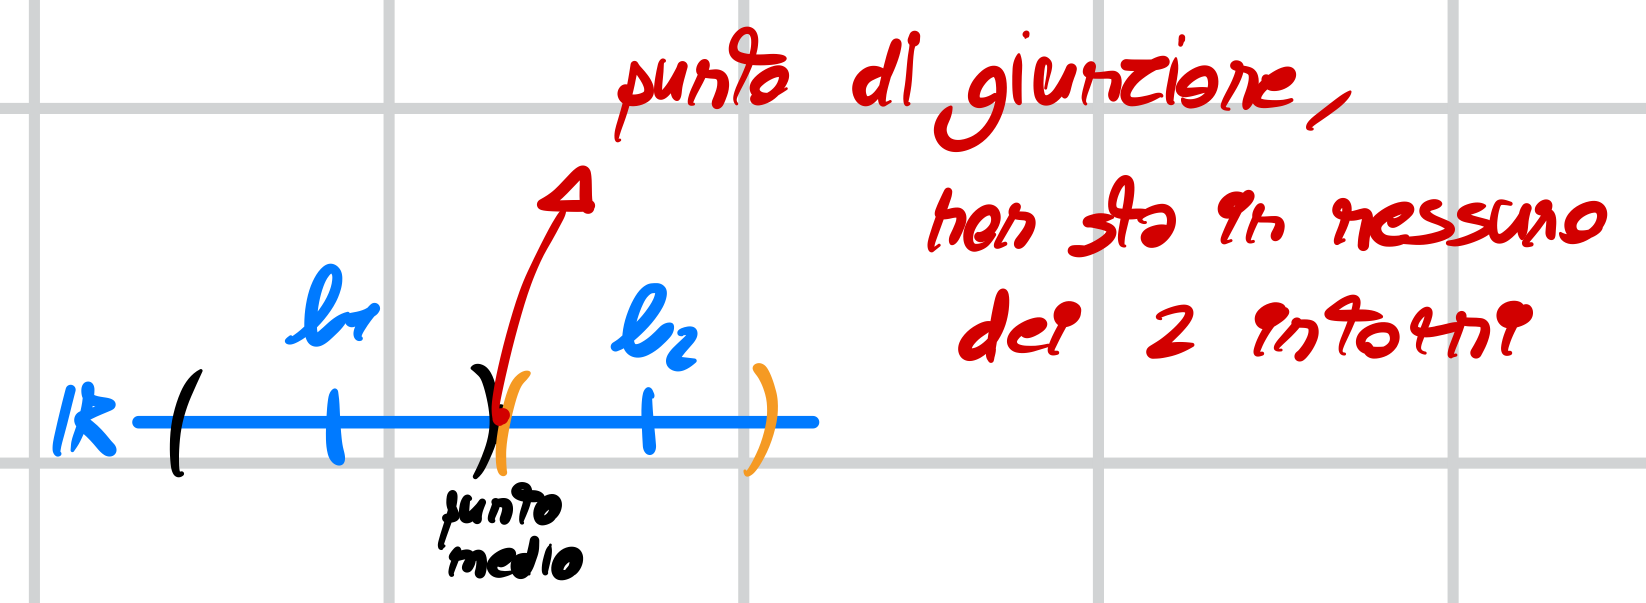
\includegraphics[width=10em]{./images/unicitaLimite.PNG}
\end{figure}

Per contraddizione: $l_1 \neq l_2$
\\Allora $\exists Vl_1, Vl_2$ intorni di $l_1$ e $l_2$ (rispettivamente) tali che: $Vl_1 \bigcup Vl_2 \neq \emptyset$
\\$Wx_0 = \bigcup U'x_0$ è un intorno di $x_0$
\\Sia $x \in(Wx_0 \bigcup A) - \{x_0\} \neq \emptyset$ (perché $x_0$ è di accumulazione)
\[
    \Rightarrow
    \begin{cases}
        f(x) \in Vl_1 \text{  (Per definizione di limite 1)}\\
        f(x) \in Vl_2 \text{  (Per definizione di limite 2)}
    \end{cases}
\]
\[
    \Rightarrow f(x) \in Vl_1 \bigcap Vl_2 \neq \emptyset \Rightarrow \mathbf{l_1 = l_2}. \mathbf{\textbf{ \underline{Contraddizione}}}
\]

\section{Teorema fondamentale del calcolo integrale (TFCI)} \label{TFCI}
\subsection{Enunciato}
$[a,b] \subset \R$, $a < b$. $f$ R-integrale su $[a,b]$.
\\$\exists x_1 \in [a,b]$ t.c. $f$ sia continua in $x_1$.
\\Fissato $x_0 \in $[a,b] e presa $F(x) = \int_{x_0}^{x}f(t)dt$, si ha che $F$ è derivabile in $x_1$ e $F'(x_1)=f(x_1)$
\subsection{Dimostrazione}

\begin{align*}
    0 &\leq \left| \frac{F(x) - F(x_1)}{x - x_1} - f(x_1) \right|, \quad x \neq x_1 \\
    &= \left| \frac{\int_{x_0}^{x} f(t) dt - \int_{x_0}^{x_1} f(t) dt}{x - x_1} - f(x_1) \right| \\
    &= \left| \frac{\int_{x_0}^{x} f(t) dt + \int_{x_1}^{x} f(t) dt - \int_{x_0}^{x_1} f(t) dt}{x - x_1} - f(x_1) \right| \\
    &= \left| \frac{\int_{x_1}^{x} f(t) dt - f(x_1)(x - x_1)}{x - x_1} \right| \\
    &= \left| \frac{\int_{x_1}^{x} (f(t) - f(x_1)) dt}{x - x_1} \right| \\
    &\leq \frac{1}{x - x_1} \int_{x_1}^{x} |f(t) - f(x_1)| dt
\end{align*}
\Space
\\Ma $f$ è continua in $x_1 \iff $
\[\forall\epsilon>0\text{ }\exists \DeltaEp>0\text{ t.c. }\left|f(t) - f(x_1)\right|<\epsilon\text{ }\forall t / 0 < \left|t-x_1\right|<\DeltaEp\text{ }t\in[a,b]\]
Osservo che $t\in[x_1, x]$ (oppure $t\in[x, x_1]$, dipende come abbiamo disposto $x$ e $x_1$)
\\Implica che $\left|t-x_1\right| \leq \left|x - x_1\right|$
\\Sia allora $x\in[a, b] / \left|x-x_1\right|<\DeltaEp$. \underline{Con questo forziamo le due varibli a stare vicine fra loro}
\\Quindi $\left|t-x_1\right| \leq \left|x-x_1\right|<\DeltaEp$ e $\left|f(t) - f(x_1)\right|<\epsilon$
\\Allora $0\leq\left|\frac{F(x)-F(x_1)}{x-x_1}-f(x_1)\right| < \frac{1}{\left|x-x_1\right|}\left|\int_{x_1}^{x}\epsilon dt\right| = \epsilon \frac{\left|x-x_1\right|}{\left|x-x_1\right|} = \epsilon$
\\Ossia: $\forall \epsilon > 0$ $\exists \DeltaEp > 0$ t.c. $\left|\frac{F(x)-F(x_1)}{x-x_1}-f(x_1)\right|<\epsilon$ $\forall x$ t.c. $0<\left|x-x_1\right|<\DeltaEp$, $x\in[a,b]$
\\Cioè:$\lim_{x_1}\frac{F(x)-F(x_1)}{x-x_1}$ esiste e vale $f(x_1)$.
\\\begin{center} \textbf{Quindi: $\mathbf{F'(x_1) = f(x_1)}$}\end{center}

\section{Formula fondamentale del calcolo integrale}
\subsection{Enunciato}
$f \in C^0[a,b]$ e sia $G : [a,b] \rightarrow {\R}$ una primitiva di $f$ in $[a,b]$
\\\begin{center}Allora $\int_{a}^{b}f(t)dt = G(b) - G(a)$\end{center}

\subsection{Dimostrazione}
Sia $x \in [a,b]$ e $F(x)= \int_{x_0}^{x}f(t)dt$. Per il TFCI* è derivabile in $[a,b]$ e $F'(x)=f(x) \forall x \in [a,b]$.
\\$F$, $G$ sono primitive di $f$ in un intervallo $[a,b] \Rightarrow$ $\exists c \in {\R} /G(x)=F(x)+c$ $\forall x \in [a,b]$
\begin{center}
    Osservo adesso che: $G(b) - G(a) = F(b)+c-F(a)-c=F(b)-F(a)$
    \\$= \int_{x_0}^{b}f(t)dt - \int_{x_0}^{a}f(t)dt$
    \\$= \cancel{\int_{x_0}^{a}f(t)dt} + \int_{x_0}^{b}f(t)dt - \cancel{\int_{x_0}^{a}f(t)dt} = \int_{x_0}^{b}f(t)dt$.
\end{center}
*TFCI: \hyperref[TFCI]{Teorema Fondamentale Calcolo Integrale}
\Space
\\\underline{\textbf{Osservazione:}} $f \in C^0 ([a,b])$ e sia
\\$H(x) = \int_{\alpha(x)}^{\beta(x)}f(t)dt$ dove $\alpha,\beta:[a,b]\rightarrow \R$ derivabili in $[a,b]$.
\\Si ha che $H(x)$ è derivabile perché $H(x)=F(\beta(x))-F(\alpha(x))$ dove $F(u)=\int_{x_0}^{u}f(t)dt$ \textit{(Composizione di $f$ derivabili)}
\\Inoltre $H'(x)=F'(\beta(x))\beta'(x) - F'(\alpha(x))\alpha'(x) = $ \underline{$f(\beta (x))\beta'(x)-f(\alpha(x))\alpha'(x)$ $\forall x \in [a,b]$}


\section{Teorema del confronto I}
\subsection{Enunciato}
$f, g: A \subset \R \rightarrow \R, x_0 \in \Rext$ punto di accumulazione per $A$
\\Allora: 

\begin{enumerate}
    \item[a)] Se \( \lim\limits_{x \to x_0} f(x) = \ell_1 \in \mathbb{R} \) \\
          Se \( \lim\limits_{x \to x_0} g(x) = \ell_2 \in \mathbb{R} \) \\
          con \( \ell_1 < \ell_2 \), allora:
          \[
          \exists U_{x_0}, \text{ intervallo di } x_0, \text{ tale che } f(x) < g(x) \quad \forall x \in (U_{x_0} \cap A) \setminus \{x_0\}
          \]
    
    \item[b)] Se \( \lim\limits_{x \to x_0} f(x) = -\infty \) \\
          Se \( \lim\limits_{x \to x_0} g(x) = \ell \in \mathbb{R} \cup \{+\infty\} \), allora:
          \[
          \exists U_{x_0}, \text{ intervallo di } x_0, \text{ tale che } f(x) < g(x) \quad \forall x \in (U_{x_0} \cap A) \setminus \{x_0\}
          \]

    \item[c)] Se \( \lim\limits_{x \to x_0} f(x) = \ell \in \mathbb{R} \) \\
          Se \( \lim\limits_{x \to x_0} g(x) = +\infty \), allora:
          \[
          \exists U_{x_0}, \text{ intervallo di } x_0, \text{ tale che } f(x) < g(x) \quad \forall x \in (U_{x_0} \cap A) \setminus \{x_0\}
          \]
\end{enumerate}

\subsection{Dimostrazione}
\begin{enumerate}
    \item[a)]
    $l_1 < l_2 (l_1,l_2 \in \R)$. Fisso $\epsilon>0$\\
    $\lim\limits_{x \to x_0} f(x)=l_1 \Rightarrow \exists U' x_0$ intervallo di $x_0$ tale che $\forall x \in (U' x_0 \cap A)\setminus \{x_0\}$
    \\$\lim\limits_{x \to x_0} g(x) = l_2 \Rightarrow \exists U'' x_0$ intorno di $x_0 / l_2 - \epsilon < g(x) < l_2 + \epsilon$ $\forall x \in (U'' x_0 \cap A) \setminus \{x_0\}$
    \Space
    \\Se $x \in (U' x_0 \cap U'' x_0 \cap A) \setminus \{x_0\}$ \textit{idea: scelgo $\epsilon>0 / l_1 + \epsilon \leq l_2 - \epsilon$}
    \\Scelgo in quanto sopra $\epsilon = \frac{l_2 - l_1}{2}$
    \\Per $x \in (U' x_0 \cap U'' x_0 \ cap A) \setminus \{x_0\}$ si ha allora 
    \[f(x) < l_1 + \epsilon = l_1 + \frac{l_2 - l_1}{2} = \frac{l_1 + l_2}{2}\]
\end{enumerate}

\vspace{5em}

\section{teorema del confronto II}
\subsection{Enunciato}
$f, g: A \subset \R \rightarrow \R$ $A \neq \emptyset$ $x \in \Rext$ punto di accumulazione per $A$ Allora:
\begin{enumerate}
        \item[a)]
        Se $\lim\limits_{x \to x_0} f(x) = l_1 \in \R$
        \\Se $\lim\limits_{x \to x_0} g(x) = l_2 \in \R$
        \\Se $\exists U x_0$ intorno di $x_0 / f(x) \leq g(x)$ $\forall x \in (U x_0 \cap A)\setminus \{x_0\}$
        \[\Rightarrow l_1 \leq l_2\]

        \item[b)]
        Se $\lim\limits_{x \to x_0} g(x) = - \infty$ e $\exists U x_0$ intorno di $x_0 / f(x) \leq g(x)$ $\forall x \in (U x_0 \cap A) \setminus \{x_0\}$
        \[ \Rightarrow \exists \lim\limits_{x \to x_0} g(x) = + \infty \]

        \item[c)]
        Se $\lim_limits_{x \to x_0} f(x) = + \infty$ e $\exists U x_0$ intorno di $x_0 / f(x) \leq g(x)$ $\forall x \in (U x_0 \cap A) \setminus \{x_0\}$
        \[ \Rightarrow \exists \lim\limits_{x \to x_0} g(x) = + \infty \]
\end{enumerate}
\subsection{Osservazione}
Cosa accade se si suppone $f(x) < g(x) \overset{?}{\Rightarrow} l_1 < l_2$
\[ 
    \textbf{NO: } f(x)=0 \text{ } \forall x \R \text{ } g(x) = 
    \begin{cases}
        \frac{1}{x} \text{ } x > 0\\
        0 \text{ } x = 0\\
        - \frac{1}{x} \text{ } x < 0
    \end{cases}
\]

\begin{figure}[h]
    \centering
    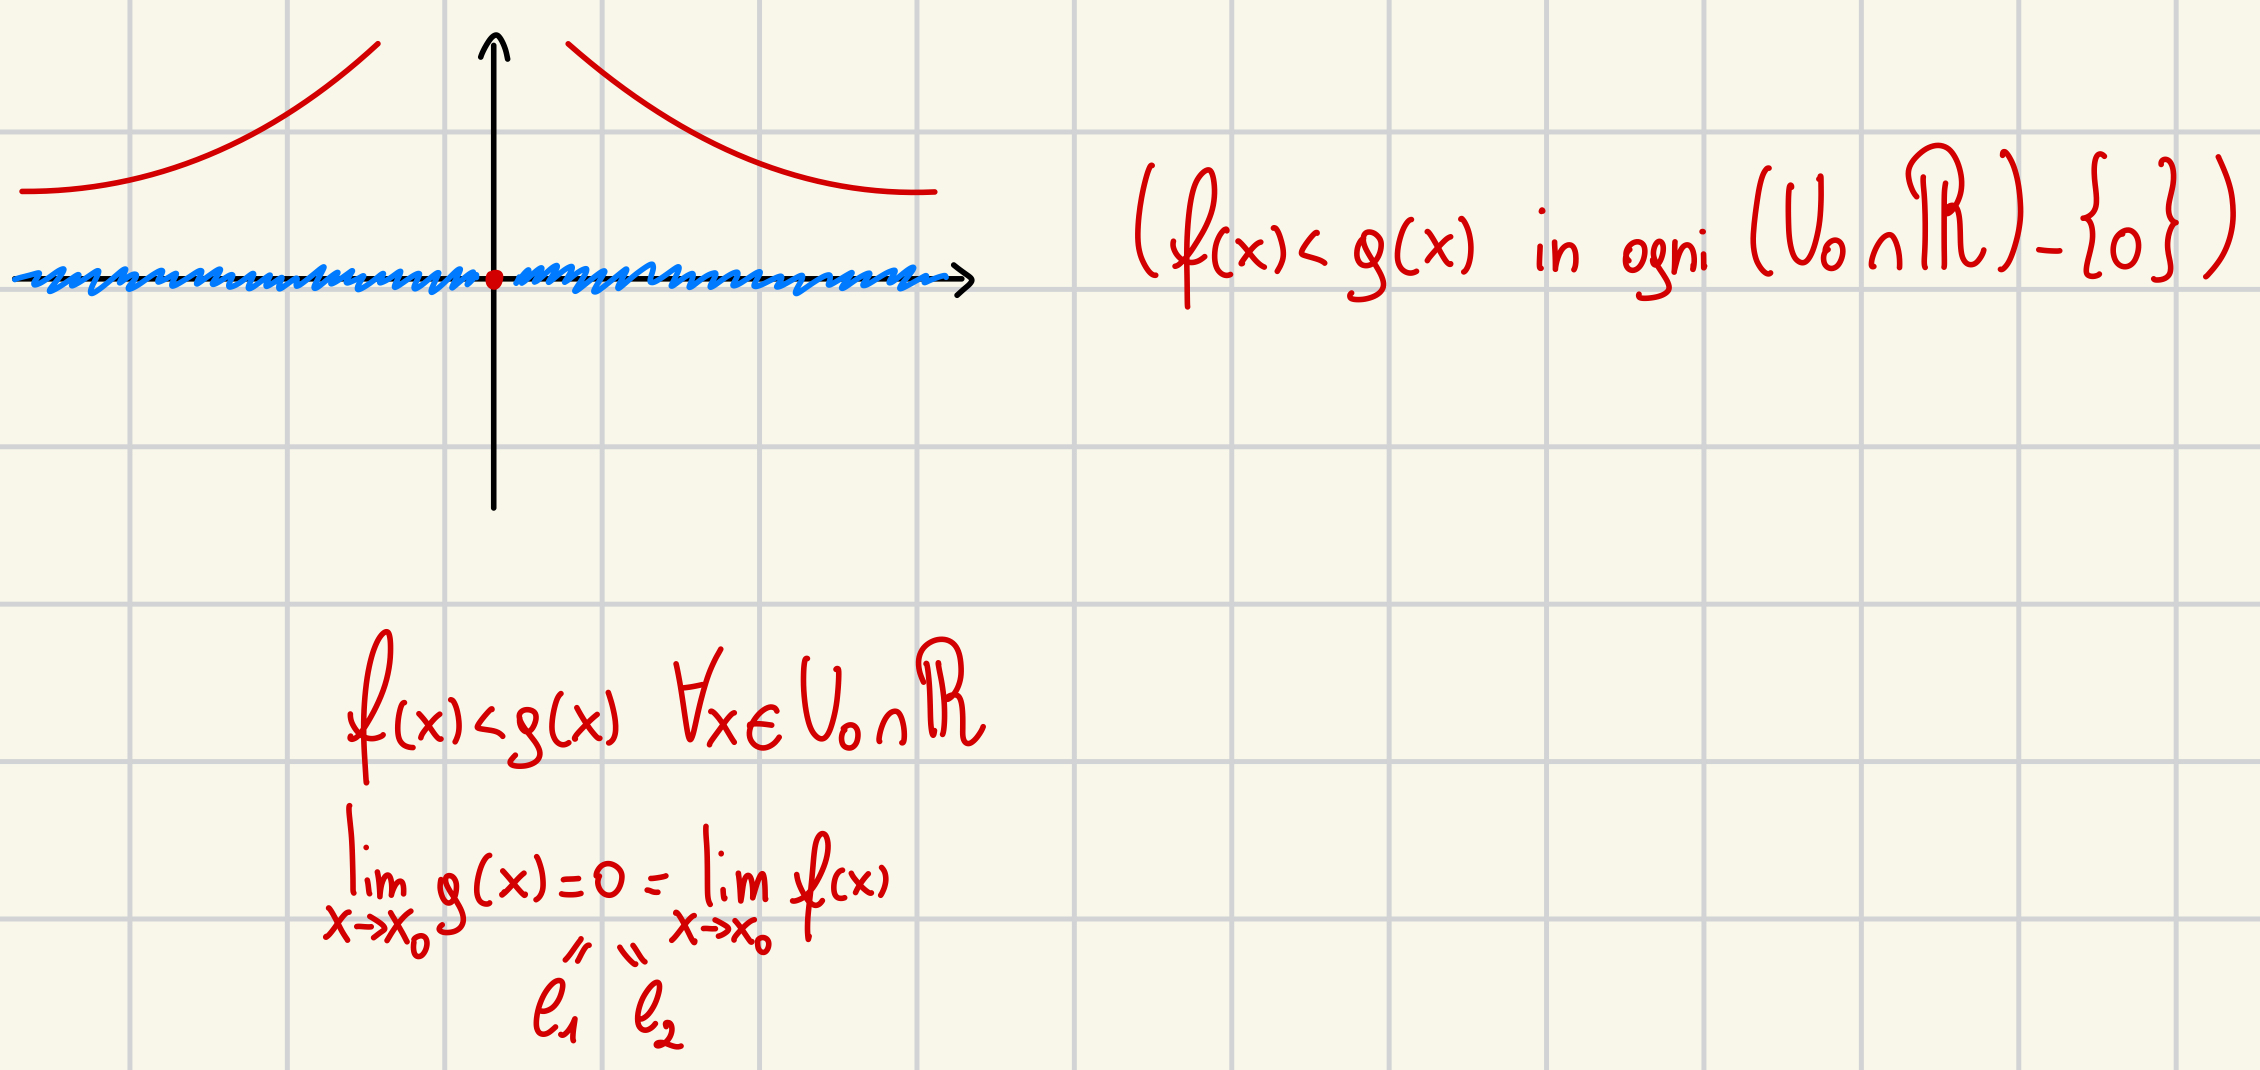
\includegraphics[width=35em]{./images/Teoriaconfronto2.jpeg}
\end{figure}

\section{Teorema del confronto dei limiti}
\section{Teorema media integrale}
\section{Condizione necessaria del primo ordine per punti estremali interni}
\section{Criterio integrale convergenza delle serie numeriche}
\subsection{Enunciato}
$f: [1, + \infty ) \rightarrow \R,$ $f(x) \geq 0$ $\forall x \in [1, + \infty$.
\\Sia $f$. debolmente crescente in $[\, + \infty )$.
\\Allora ($\sum\limits_{k=1}^{\infty} f(k)$ converge $\iff$ $\int_{1}^{+ \infty} f(x) dx$ converge.)

\section{Teorema del valore medio integale}

\section{Teorema delle 3 funzioni (Carabinieri)}

\includegraphics[width = 5em]{./images/carabinieri.png}
\subsection{Enunciato}
$f, g, h:$ $A \subset \R \rightarrow \R,$ $A \neq \emptyset,$ $x_0 \in \Rext$ punto di accumulazione per $A$.
\\Inoltre
\begin{enumerate}
    \item[] $\exists \lim\limits_{x \to x_0} f(x) = l \in \R$ 
    \item[] $\exists \lim\limits_{x \to x_0} g(x) = l \in \R$
    \item[] $\exists U x_0$ intorno di $x_0 / f(x) \leq h(x) \leq g(x)$ $\forall x \in (U x_0 \cap A) \setminus \{x_0\}$
\end{enumerate}
\[ \Rightarrow \exists \lim\limits_{x \to x_0} h(x) = l \]

\vspace{50em}

\subsection{Dimostrazione}
Sia $\epsilon > 0$: $\exists U' x_0$, $U'' x_0$ intorni di $x_0 / \left|f(x) - l\right| < \epsilon$  $\forall x \in (U' x_0 \cap A) \setminus \{x_0\}$
\\\hspace*{16.32em} $\left|g(x) - l\right| < \epsilon$  $\forall x \in (U'' x_0 \cap A) \setminus \{x_0\}$
\\\Space Sia $W x_0 = U' x_0 \cap U'' x_0$ è un intorno di $x_0$.
\\Se $x \in W x_0 \cap A \setminus \{x_0\}$
\Space
\\\hspace*{18em}$l - \epsilon < f(x)$ \underline{definizione $\lim f$ (per ipotesi)}
\\\hspace*{18em}\hspace*{3.3em}$f(x) \leq h(x) \leq g(x)$
\\\hspace*{18em}\hspace*{9.8em}$g(x) < l + \epsilon$
\Space
\\Quindi $l - \epsilon < h(x) < l + \epsilon$ cioè $\left|h(x) - l\right| < \epsilon$
\\Ho fatto vedere che:
\[
    \forall \epsilon > 0 \text{ } \exists W x_0 \text{ intorno di } x_0 / \left|h(x) - l\right| < \epsilon \text{ per } x \in W x_0 \cap A \setminus \{x_0\}
\]
\\Che è esattamente la definizione di: $\lim\limits_{x \to x_0} h(x) = l$

\section{Condizione estremalità locale con le derivate successive}


\section{Teorema di Rolle} \label{Rolle}
\subsection{Enunciato}
$f:[a,b] \rightarrow \R$, $f$ continua in $[a,b]$
\\$f$ derivabile in $(a,b)$ e $f(a) = f(b)$
\\Allora $\exists \overline{x} \in [a,b]$
\\\underline{$x_1 = a$ e $x_2 = b$ (o viceversa)}: allora, dato che
\[
    \begin{array}{c}
        f(a) = f(b) \Rightarrow f(x) = f(a) \text{ } \forall x \in [a,b] \\
        \Rightarrow f'(x) = 0 \text{ } \forall x \in (a,b)
    \end{array}
\]
Se almeno uno tra $x_1$ e $x_2$ non è in un estremo di $[a,b]$
\\esempio sia $x_1 \in (a,b)$. Allora $x_1$ è interno ad $[a,b]$. Per le condizioni necessarie di estremalità si ha $f'(x_1) = 0$
\\Nel caso di $x_2 \in (a,b)$: si replichi lo stesso ragionamento.

\section{Teorema di Lagrange}
\subsection{Enunciato}
$f:[a,b] \rightarrow \R$, $f$ continua in $[a,b]$, $f$ derivabile in $(a,b)$.
\\Allora $\exists \overline{x} \in (a,b) / f(b) - f(a) = f'(\overline{x}) (b-a)$
\\Sia $\varphi (x) = (f(x)- f(a))(b - a) - (f(b) - f(a))(x-a)$, $f$ è continua in $[a,b]$;
\\$\varphi$ è derivabile in $(a,b)$, $\varphi (a) = 0 - 0 = 0$; $\varphi (b) = 0 - 0 = 0$.
\\Per il teorema di \hyperref[Rolle]{Rolle}: $\exists \overline{x} \in (a,b)$ \hspace*{2em} $\varphi (\overline{x}) \rightarrow$ punto che azzera la derivata prima.
\\Ma $\varphi ' (x) = (f'(x)(b-a)) - (f(b)-f(a))$ $\forall x \in (a,b)$
\[
    \begin{array}{c}
        \Rightarrow 0 = \varphi ' (\overline{x}) = f'(\overline{x})(b-a) - f(b)-f(a) \\
        \text{e quindi } 0 = \varphi ' (\overline{x}) \text{ dato che il resto è nullo}\\
        \text{da cui segue la tesi.}
    \end{array}
\]

\begin{figure}[h]
    \centering
    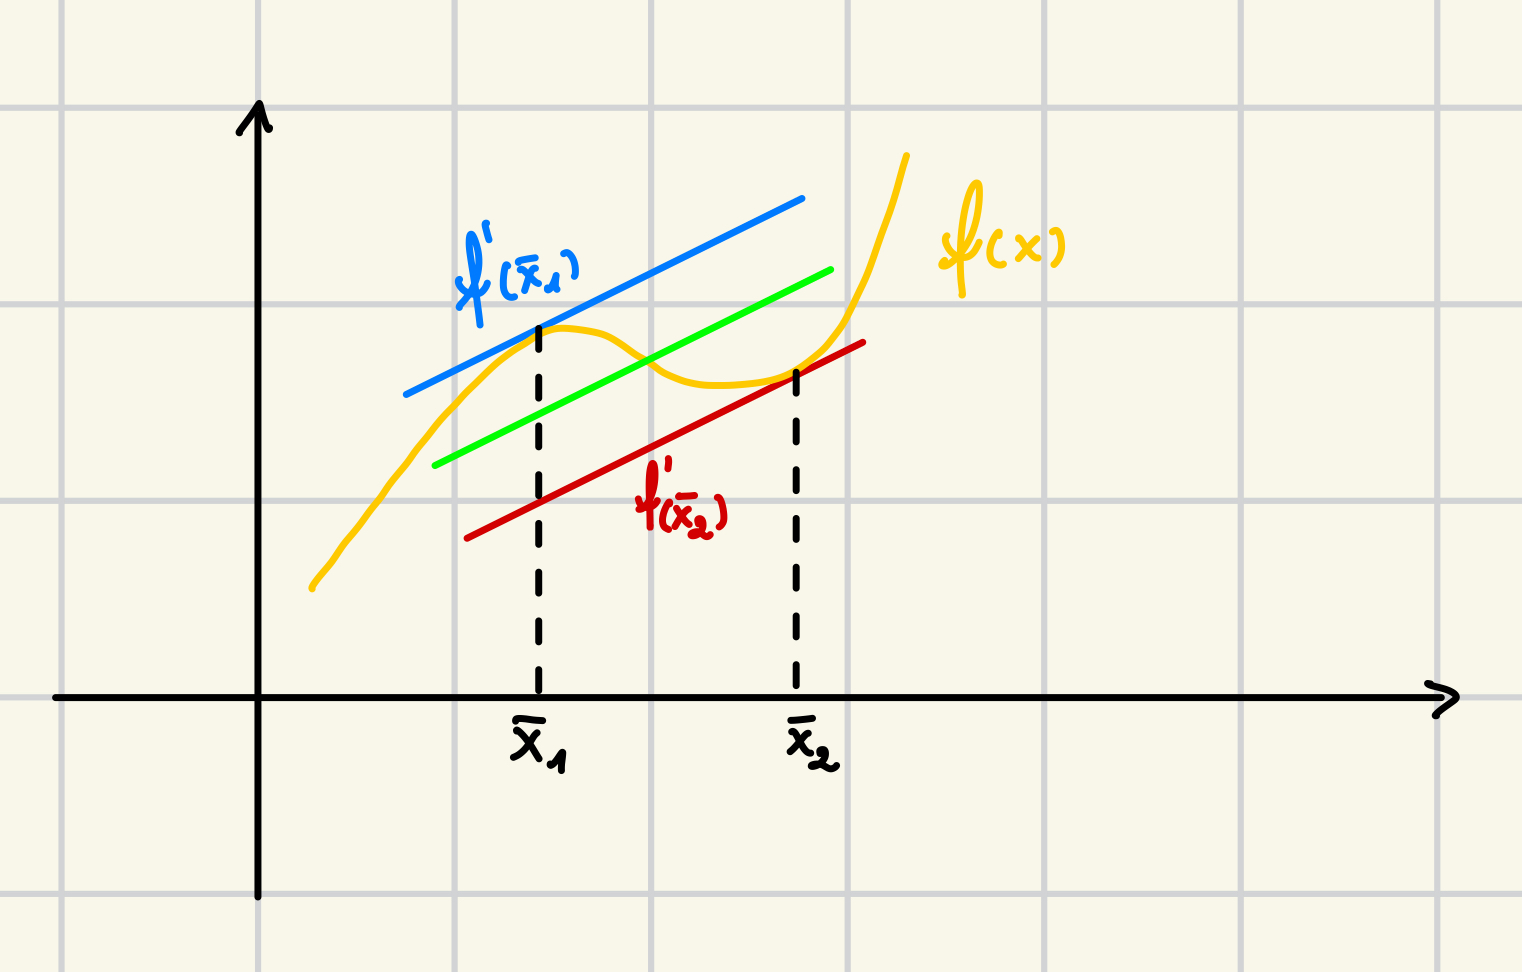
\includegraphics[width=25em]{./images/lagrange.jpeg}
\end{figure}




\end{flushleft}
\end{document}